\chapter{Conclusions}
\label{ch:conclusion}

The unification of smartphones and cameras has sparked a vast amount of applications in image processing from natural scenes. Motivated by information extraction from the unstructured data within a natural image, many applications have sought to process images via heuristics, as opposed to deep-learning neural networks, for the purposes of object detection. Potential issues begin to arise when researchers rely on heuristics. In the context of marathon runners,  facial detection is used in conjunction with a predefined ratio to determine the torso area \citep{Benami:2012jf}. In others---such as \glsx{lpr}---we find that distinct image properties (e.g., stroke, width and colour) are utilised, and thus as images become more complex, the performance is likely to degrade \citep{Li:2012wd}.

\section{Primary Contributions}

Overcoming the limitations of this \glsx{cc}-based detection strategy has been investigated within this study, by only using deep-learning \glsplx{nn} for learning-based object detection. We find that detection with learning-based methods for object detection can achieve up to 97\% accuracy using transfer-learning on pre-existing \glsx{rcnn} (\frcnn{} \citep{Ren:2017ug}) for visual processing given context of the desired object to be detected (i.e., racing bibs). We also find that transfer-learning can achieve partially similar results of up to 82\% accuracy in detection of alphanumeric regions within those extracted features by changing the dataset and desired feature to text regions.

This thesis also aimed to tackle the issue of different \glsx{ocr} strategies. We have shown that our pipeline is able to use \gls{nn}-based \gls{ocr} to recognise the alphanumeric sequences of a \glsx{rbn} without character segmentation. We also show that preprocessing these images are a requirement for non-binarised text (i.e., red \glspl{rbn}) into pre-existing \gls{ocr} engines such as Tesseract.

We define an approach to define the prominence of a given runner within a photo using a data-collection system, \textit{Argus}, that was used to curate labels for a large dataset in order to train the network. As a side research tangent of this thesis, we achieved a metamodel proposing how such applications can be used for further contexts, and not just marathon photography, as well as a metamodel development methodology to create metamodels using a quasi-experimental design and observational studies of a prototype systems.

% RQ -> Contributon

% This is what I started with, relate back to introduction and research questions
% What were the main contributions that solved the RQs?
% Everything in the pipeline is generally reusable, except for training images and OCR NN font training.

\section{Future Work}

Our end-to-end \gls{nn} pipeline shows significant fallbacks on human cropping---the proposed method of introducing cropping to improve accuracies has been shown to degrade our performance, rather than the initial intention to improve it. Overcoming this limitation may be as simple as re-training \frcnn{} simply on cropped images with wider padding, rather than on raw images, though testing such a hypothesis is left open.

While we have developed a system to label the prominence of runners, we still leave the implementation of a classifier to understand what prominence is open to future work. By proposing a method by which all crowded photos are discarded and teaching a classifier on biased \glsx{lop} (i.e., by removing the intermediary \textsc{maybe} candidates), such prominence ranking of subjects is within reach.

Similarly, the degrading text area detection may be improved by applying transfer learning to other \gls{rcnn}-based networks on a per-pixel level. As mentioned in \cref{sec:background:detection:learning}, Mask-\gls{rcnn}, has recently appeared as a preprint in early \citeyear{He:2017ud}. Improvements to Argus to record data points on a per-pixel basis may allow for improvement in the areas of per-pixel detection, thereby extracting digits from a \gls{rbn} within a bib even easier. An illustration of potential such applications are shown in \cref{fig:conclusion:future_work:mask_rcnn}.

We propose to mitigate this bottleneck limitation of poor character detection by applying transfer learning to \frcnn{} in a similar fashion to that described in \cref{sec:processing_pipeline:bib_detection:deep_learning}. By producing a synthetic \gls{rbn} dataset similar to that of \citet{Jaderberg:2014uy,Jaderberg:2016wj} (with ground truth bounding boxes of each character known), we can augment these sample \glspl{rbn} and therefore re-train \frcnn{} to understand positions of characters. Each character from the detected regions can be extracted and piped into a \gls{cnn} trained on recognising specific digits, or perhaps---in addition to training \frcnn{} to learn the positions of characters---the characters themselves can be trained in the same process. We leave such an implementation open to future works.

\begin{figure}
  \centering
  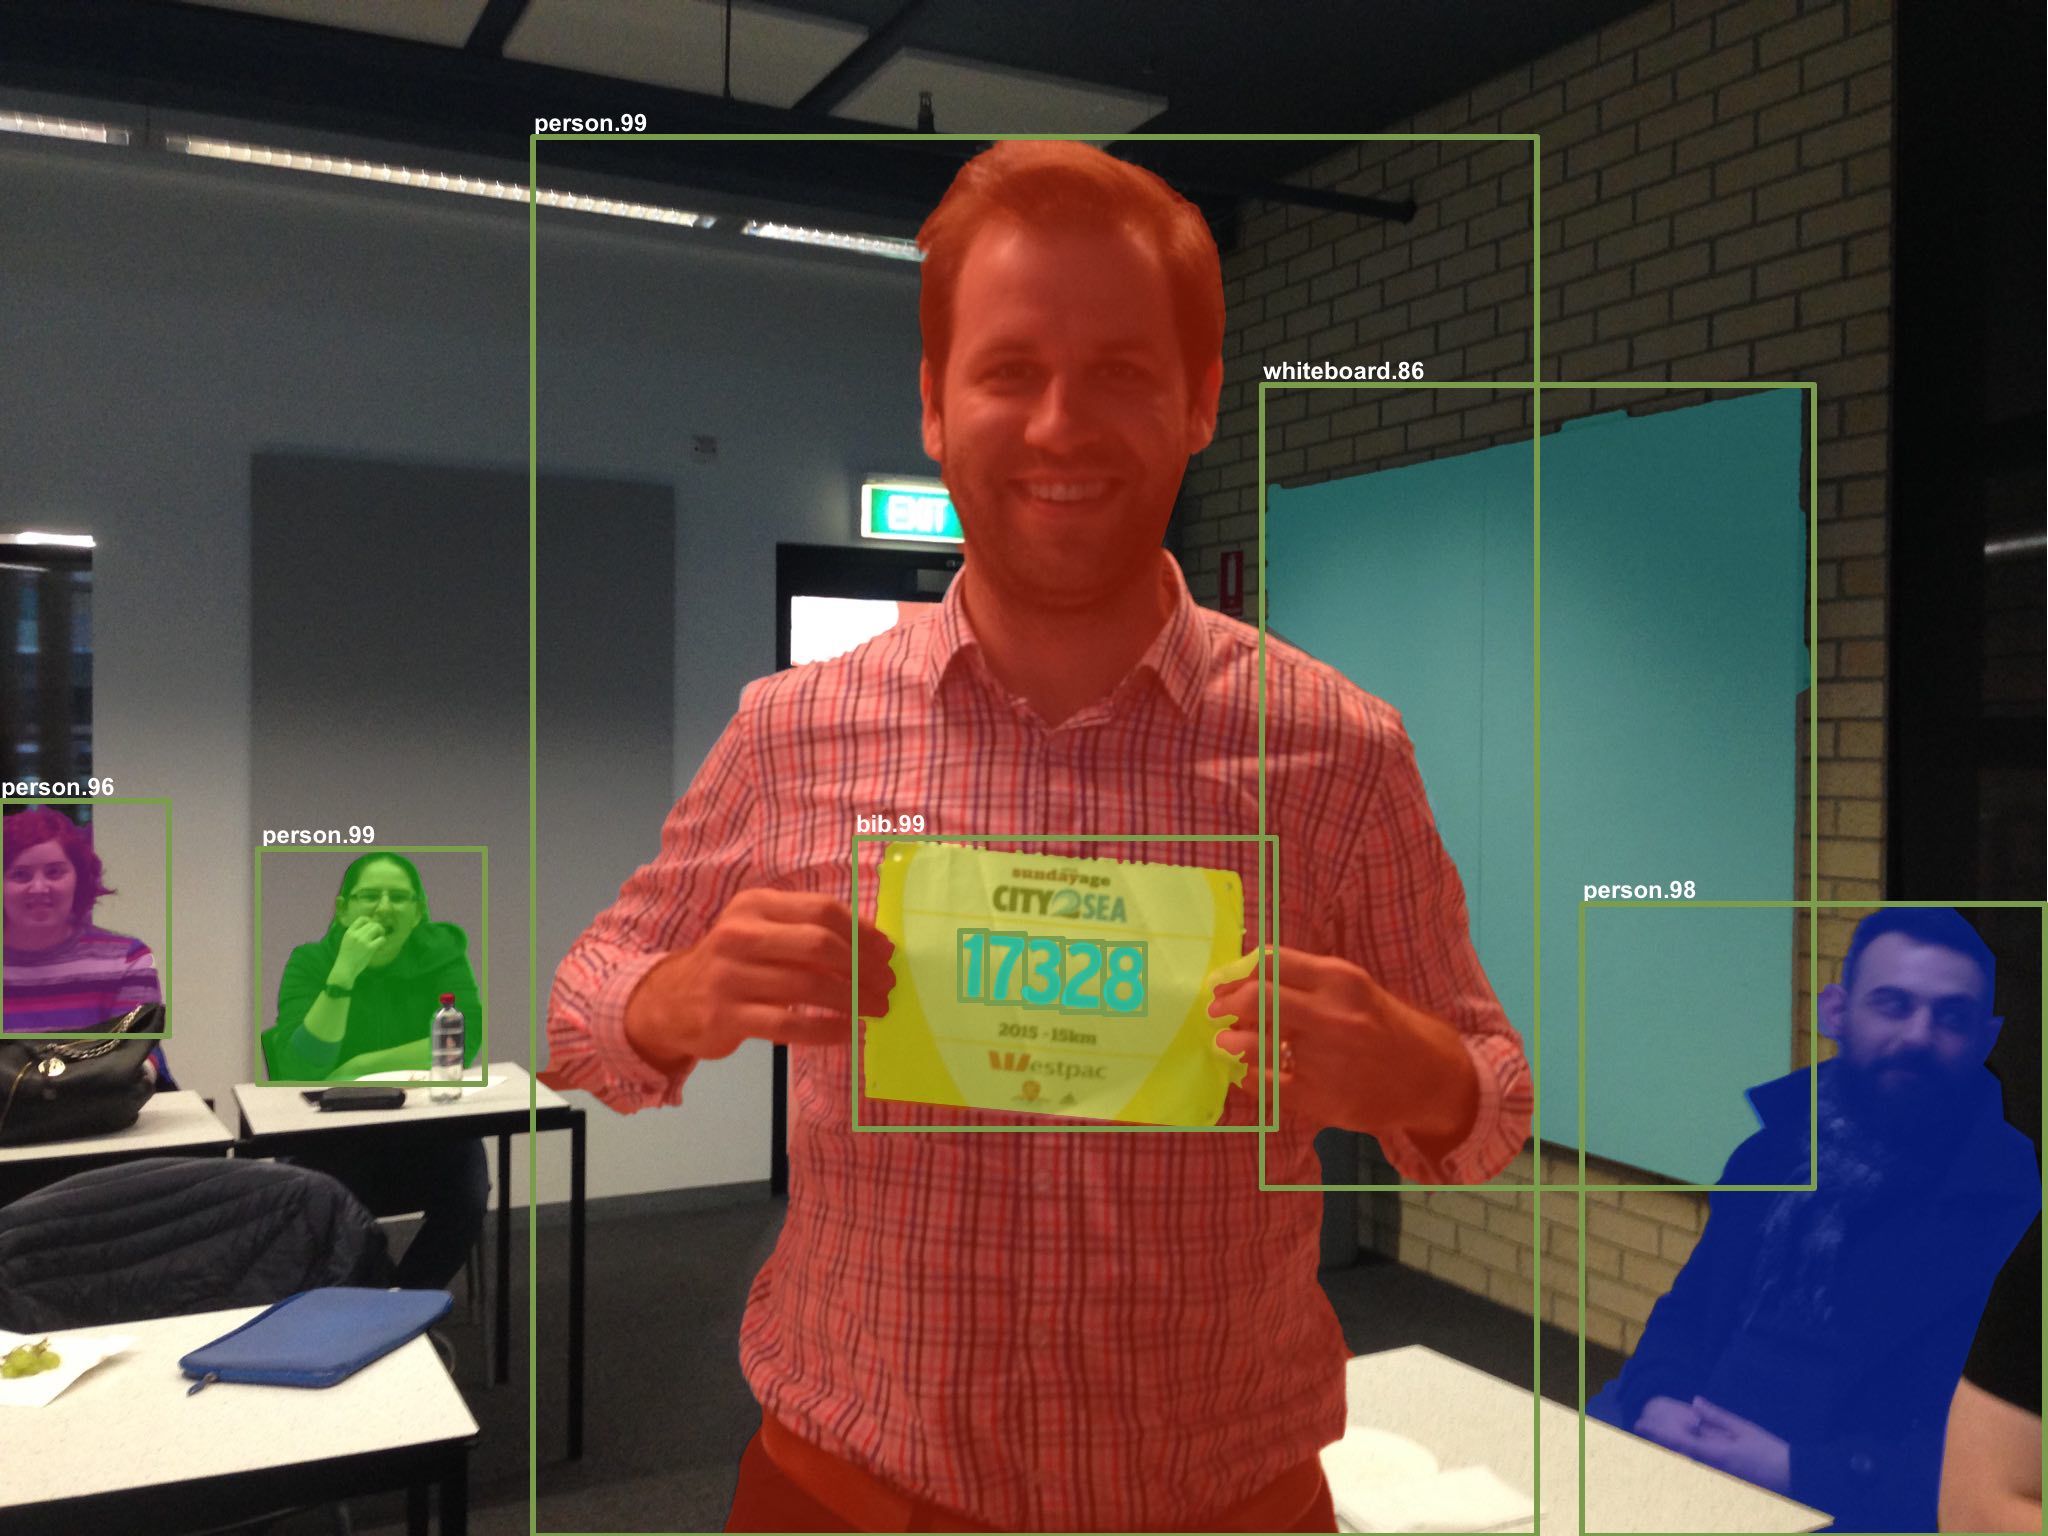
\includegraphics[width=0.9\textwidth]{images/conclusion/mask-rcnn}
  \caption[Potential use of Mask-RCNN on to recognise an RBN]{Potential use of Mask \gls{rcnn} to detect a bib sheet and its \gls{rbn} on with per-pixel accuracy.}
  \label{fig:conclusion:future_work:mask_rcnn}
\end{figure}

\section{Wider Applicability}

Alphanumeric character recognition goes far beyond \gls{rbn} recognition. Other contexts in the area of self-driving vehicle literature, such as \gls{lpr} and \glsx{tsr}, is imperative for the realisation of these vehicles. Similar areas include meter reading of electronic and water meters, or street sign numbers as discussed in \cref{ch:background}. 

The objective is to change the feature of interest: if one is interested in training a network about license plates, then train the network as we have done with racing bib numbers, but with an annotated dataset labelled with license plates. Additionally, training a text detection network with typeface specificity in mind (i.e., if one knows the typeface of a license plate or electronic meter), swapping out the text recognition portion of our pipeline with this trained network is achievable. This can be done to not only improve our \gls{ocr} bottleneck, but to improve context-specific cases.

% Runtime speed improvements
%% Where was the biggest bottleneck? Engineering of Keras FRCNN to be improved architecturally to always be running on a all image basis, not spin up one per image

% OCR improvements
%% Use a NN to detect text better on a per-character basis.
%% Train a NN with domain-specific font. E.g., Vic License Plate typeface, typeface for electric box readers

% Wider applicability (other contexts)
%% Speed limit signs
%% License plate recognition
%% Electric box/water meters
%% Use a NN to train the OCR for font-specific applicability

\section{Closing Remarks}

In his \citeyear{Schwab:2017vd} book, \citet{Schwab:2017vd}, the founder and executive chairman of the World Economic Forum, discusses the impact on human society with the impending fourth industrial revolution, coined Industry 4.0 by \citet{kagermann2011industrie}. Schwab discusses that such a revolution will fundamentally be underpinned by \glsx{ai} systems. Thus, improvements in object detection, prominence ranking, and alphanumeric sequence recognition are just a slice of how the impact of automation may lessen the need for humanity to rely on heuristic-driven systems.

% General wrap-up
\bigskip
\noindent
We anticipate that this thesis encompasses the body of how \gls{ai} systems, like the pipeline developed within this work, show that we are only at the beginning for what is soon to come\ldots